\chapter{Training des BNNs}
Wie bereits in Kapitel \ref{sec:training} beschrieben, werden Netzwerke über eine rechenintensive Annäherung der Kantengewichte an das optimale Ergebnis trainiert. Diese Konvergenz in Richtung eines besseren Ergebnisses kann hierbei, selbst bei schlechtem Training, meist erreicht werden, da selbst marginale Verbesserungen eine Auswirkung haben. Da \textit{BNNs} jedoch die stärkste Form von quantisierten Netzwerken sind, können hier keine stetigen Änderungen an den Kantengewichten vorgenommen werden. Somit ist Abstimmung der Trainingsparameter essentiell.
\section{Lernrate}
Die Lernrate ist ein zentrales Parameter beim Training von Neuronalen Netzwerken. Sie gibt die Rate an, mit der Kantengewichte in einem Durchlauf angepasst werden. Je höher die Lernrate also ist, desto schneller passt sich das Model an gerade trainierte Daten an. Bei der Wahl der Rate sind die Probleme des \textit{overfitting} und \textit{underfitting} zu beachten.\\ 
Als \textit{undefitting} bezeichnet man eine zu geringe Anpassungsfähigkeit des Netzwerkes, ausgelöst über zu kleine Netze oder zu niedrige Lernrate. Ist die Lernrate zu klein, kann der Error nicht reduziert werden, die Genauigkeit nimmt nur, wenn überhaupt, sehr langsam zu. Das Netz kann aus Daten keine Lernerfolge ziehen.\\
\textit{Overfitting} ist eine zu schnelle Anpassung des Models. Ist zum Beispiel die Lernrate zu hoch, kann die optimale Genauigkeit des Netzwerkes nicht erreicht werden, da die Anpassungen pro Error-Berechnung zu groß sind. Hier wird das Optimum immer, durch eine Überkorrektur, übersprungen und kann nie erreicht werden\cite{smith2018}. Diese Probleme sind hier analog zu \textit{vanishing-} beziehungsweise \textit{exploding gradient}.

\begin{figure}[H]
	\centering
	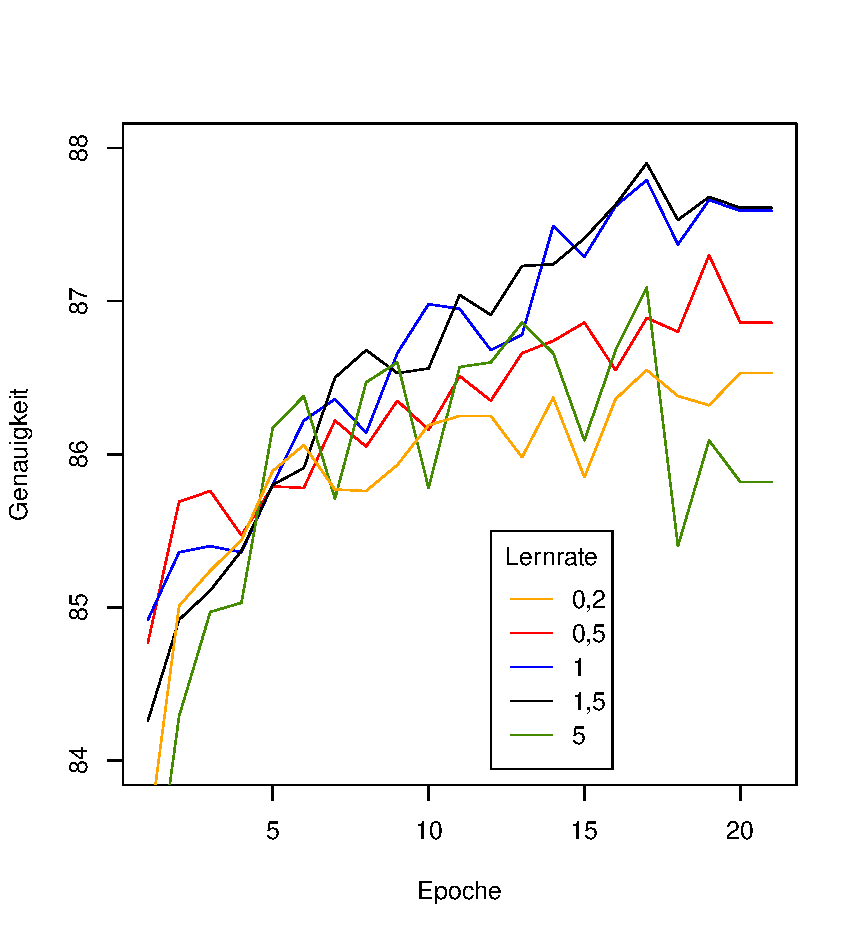
\includegraphics[scale=0.9]{./bilder/learningrate}
	\caption{Training mit verschiedenen Lernraten}
	\label{fig:learningrate}
\end{figure}

Zur Ermittlung der optimalen Lernrate haben wir unser Netzwerk für 20 Epochen mit verschiedenen Lernraten trainieren lassen. In Abbildung \ref{fig:learningrate} sind die Ergebnisse mit einer Messung der Genauigkeit nach jeder Epoche dargestellt. Bei einer Lernrate von 5 ist deutlich eine Überkorrektur ab Generation 17 zu erkennen. Hier werden zu starke Anpassungen vorgenommen, weshalb sich die Genauigkeit vom Optimum entfernt. Lernraten unter Eins hingegen nähern sich dem Optimum erst gar nicht genug an. Hier ist ein potentieller \textit{vanishing gradient} zu erkennen, da der Error nicht signifikant sinkt.  Die Lernraten 1 und $1,5$ liefern hier die besten Ergebnisse. Da das Training mit einer Rate von $1,5$ weniger große Ausschläge zeigt, wurde sich für diese Lernrate entschieden.
\section{Batchgröße}
Die Batchgröße hat Einfluss auf mehrere Punkte des Netzwerkes. Zum Einen entscheidet sie, wie viele Daten durch das Netzwerk laufen, bevor der Error gemessen wird und die Gewichte aktualisiert werden. Somit ist sie Quasi eine Rate der Error-Berechnung. Zum Anderen wirkt sich dies auf die BatchNorm Schicht aus. Je größer hier die Batchgröße ist, desto stärker ist die Normalisierung durch die BatchNorm.

\begin{figure}[H]
	\centering
	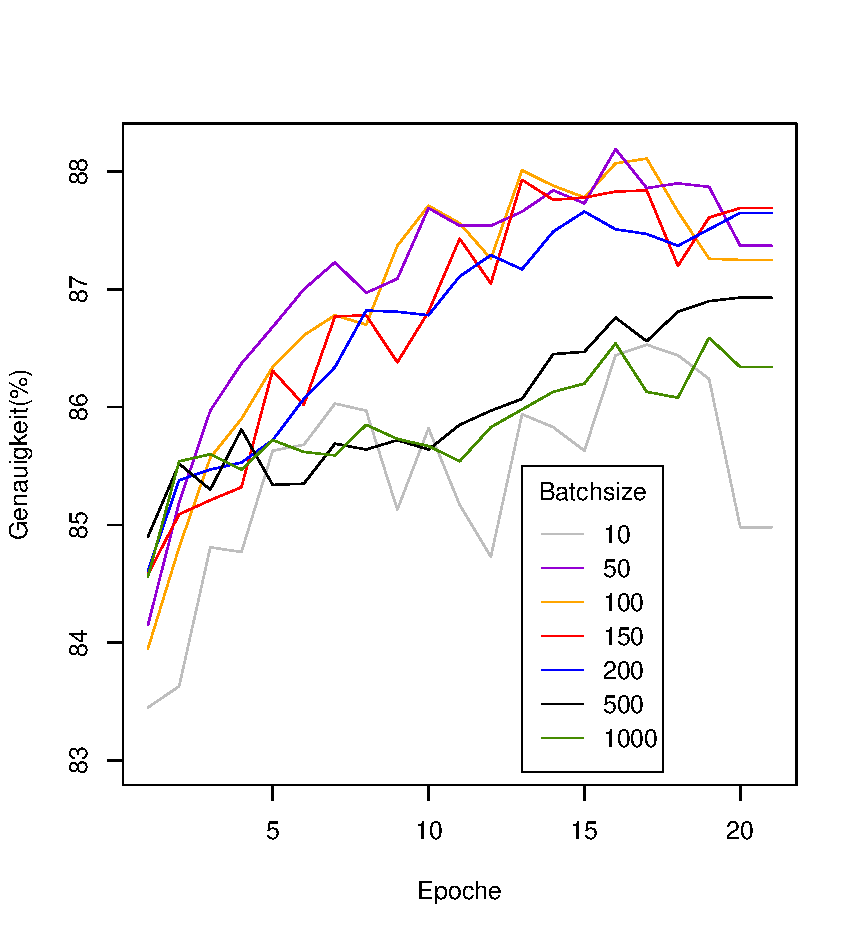
\includegraphics[scale=0.9]{./bilder/batchsize_measurement}
	\caption{Training mit verschiedenen Batchgrößen}
	\label{fig:batchsize}
\end{figure}
In Abbildung \ref{fig:batchsize} zu sehen ist das immer gleiche Netzwerk, lediglich mit angepasster Batchgröße. Dieses Netzwerk wurde für 20 Epochen beobachtet.\\
Auffällig ist die stark ausschlagende Kurve bei einer Batchgröße von 10. Hier ist der Wert zu gering, weshalb der Error oft berechnet wird. Da außerdem wenig über die BatchNorm normalisiert wird, kommt es zu hohen Error-Werten und starken und häufigen Anpassungen des Netzwerkes.\\
Bei einer Batchgröße $\geq 500$ sind weniger starke Ausschläge zu beobachten. Allerdings ist hier zu beobachten, dass das Netzwerk nicht mehr so effizient trainiert wie bei kleineren Batchgrößen. Hier könnte die Normalisierung und damit die Generalisierung bereits zu stark sein um aus einzelnen Daten überhaupt zu lernen. Außerdem wird hier der Error wesentlich seltener berechnet und das Netzwerk ist somit wesentlich unagiler. Es kommt zum \textit{underfitting}.\\
Bei Batchgrößen 50-200 ist keine besondere Abweichung zu erkennen, wobei 50 und 100 am besten performen.
\begin{figure}[H]
	\centering
	\begin{tabular}{|c|c|c|c|c|c|c|c|}\hline
		Batchgröße&10&50&100&150&200&500&1000\\\hline
		Zeit (s)&30,68&11,33&8,76&7,95&7,63&6,66&6,39\\\hline
	\end{tabular}
	\caption{Zeit pro Epoche für verschiedene Batchgrößen }
	\label{fig:batchsize_time}
\end{figure}
Ein weiterer, praxisrelevanter, Faktor ist, dass das Training mit größeren Batchgrößen schneller geht. Da mehr Daten parallel bearbeitet werden und eine GPU parallele Rechnungen gut performen kann, ist die gleiche Anzahl an Daten schneller abgearbeitet. In Abbildung \ref{fig:batchsize_time} sind die Zeiten für eine einzige Epoche, abhängig von der jeweiligen Batchgröße, gelistet. Es ist zu erkennen, dass besonders kleine Batchgrößen bei einer Erhöhung Zeiteinsparungspotential haben. Da die Werte 50-200 bei der Genauigkeit am besten abgeschnitten haben und $t(100)-t(50) <t(200)-t(100)$, ist hier die Laufzeitverbesserung von 50 auf 100 eine Sinnvolle Einsparung. Bei Batchgrößen $\geq 150$ lohnt sich die marginale Zeiteinsparung im Vergleich zur schlechteren Genauigkeit nicht mehr.\\
Deshalb haben wir uns für ein Batchgröße von 100 zur optimalen Werteberechnung entschieden.

